\section{问题四：救援任务分区与资源配置优化}

\subsection{模型建立}

问题四以问题三主方案（16 条合并路线、29 架次：运输 16 + 中继 13）为基础，将 15 个服务区划分为 $K=2$ 和 $K=3$ 个任务组。分区过程中保持问题三已确定的组批、访问顺序、运输与中继任务安排及通信保障关系不变，各组仅承担本组服务区任务并独立核算资源，资源不得跨组调配。

\subsubsection{must-link 收缩与原子任务块}

因同一运输架次涉及多个服务区时这些服务区必须同组，本文用并查集对 15 个服务区做 must-link 收缩，得到 13 个原子任务块：块 7$\{S007,S015\}$、块 8$\{S008,S011\}$ 为两个多站块，其余 11 个为单服务区块。任务分区即在 13 个不可拆分任务块上做 $K$ 组无标签划分。

\subsubsection{资源峰值并发需求核算}

对给定分区，按（任务组，资源类型）分桶，用事件扫描计算各组资源的峰值并发需求。忙碌区间口径：运输无人机 $[start,end]$、共享电池 $[start,end+t^{\rm chg}]$、中继无人机 $[depart,ground\_arrive+t^{\rm turn}]$、中继能源组件 $[depart,ground\_arrive+t^{\rm chg}]$。现有库存为：运输无人机 A/B/C 各 4/2/2 架，共享电池 A/B/C 各 6/4/4 组，中继无人机 2 架，中继能源组件 6 个，合计 30 单位。

\subsubsection{四维评价指标}

设各组资源峰值需求为 $need_{g,key}$，库存为 $inv_{key}$，则按资源 key 汇总各组需求后定义：
\begin{equation}
\begin{aligned}
Gap &= \sum_{key}\max\!\Big(0,\ \sum_g need_{g,key} - inv_{key}\Big),\\
Red &= \sum_{key}\max\!\Big(0,\ inv_{key} - \sum_g need_{g,key}\Big),\\
Bal &= \frac{\mathrm{std}(w_g)}{\mathrm{mean}(w_g)},
\end{aligned}
\end{equation}
其中 $Gap$ 为资源缺口、$Red$ 为资源冗余、$Bal$ 为组间工作量均衡系数，$w_g$ 为各组归一化工作量（作业时长 + 运输与中继能耗 + 箱数加权），$Bal$ 越小越均衡。优化按字典序 $(Gap,\ \text{总规模},\ Bal,\ Red)$ 取最优，缺口 $Gap$ 最优先。

\subsection{主方案：完全枚举精确分区}

主方案（对应代码 \texttt{q4\_1.py}）对 13 个原子块做完全枚举：K=2 枚举 $S(13,2)=4095$ 个无标签分区、K=3 枚举 $S(13,3)=261625$ 个，按同一字典序评分取全局最优，故在 13 块空间内为严格全局最优解。算法如算法~\ref{alg:q4_enum} 所示。

\begin{algorithm}[htbp]
\caption{问题四主方案：冲突图收缩 + 完全枚举精确分区（q4\_1.py）}
\label{alg:q4_enum}
\LinesNumbered
\KwIn{13 个原子任务块、问题三路线/架次/通信关系、库存}
\KwOut{K=2/K=3 全局最优分区与资源核算}
对每个无标签分区，按（任务组，资源类型）分桶，事件扫描求峰值并发需求\;
按资源 key 汇总各组需求，计算 $(Gap,\ \text{总规模},\ Bal,\ Red)$\;
按字典序 $Gap\succ\text{总规模}\succ Bal\succ Red$ 取最小者作为全局最优\;
输出分区方案、各组资源需求与缺口明细\;
\end{algorithm}

主方案结果见表~\ref{tab:q4_main} 与图~\ref{fig:q4_main_overview}。K=2 时得到 2 组分区（组 1：S001、S002、S003、S009、S012、S013；组 2：S004、S005、S006、S007、S008、S010、S011、S014、S015），资源配置总规模 18、均衡系数 0.0337、冗余 13、缺口 1；K=3 时得到 3 组分区（组 1：S001、S002、S003、S014；组 2：S004、S005、S006、S007、S008、S011、S015；组 3：S009、S010、S012、S013），总规模 21、均衡系数 0.3350、冗余 10、缺口 1。

\begin{table}[htbp]
\centering
\caption{问题四主方案（完全枚举）分区结果}
\label{tab:q4_main}
\small
\begin{tabular}{lcccc}
\toprule
\textbf{分区} & \textbf{总规模} & \textbf{均衡系数} & \textbf{冗余} & \textbf{缺口} \\
\midrule
K=2 & 18 & 0.0337 & 13 & 1 \\
K=3 & 21 & 0.3350 & 10 & 1 \\
\bottomrule
\end{tabular}
\end{table}

\begin{figure}[htbp]
\centering
\subfloat[K=2 与 K=3 分区地图]{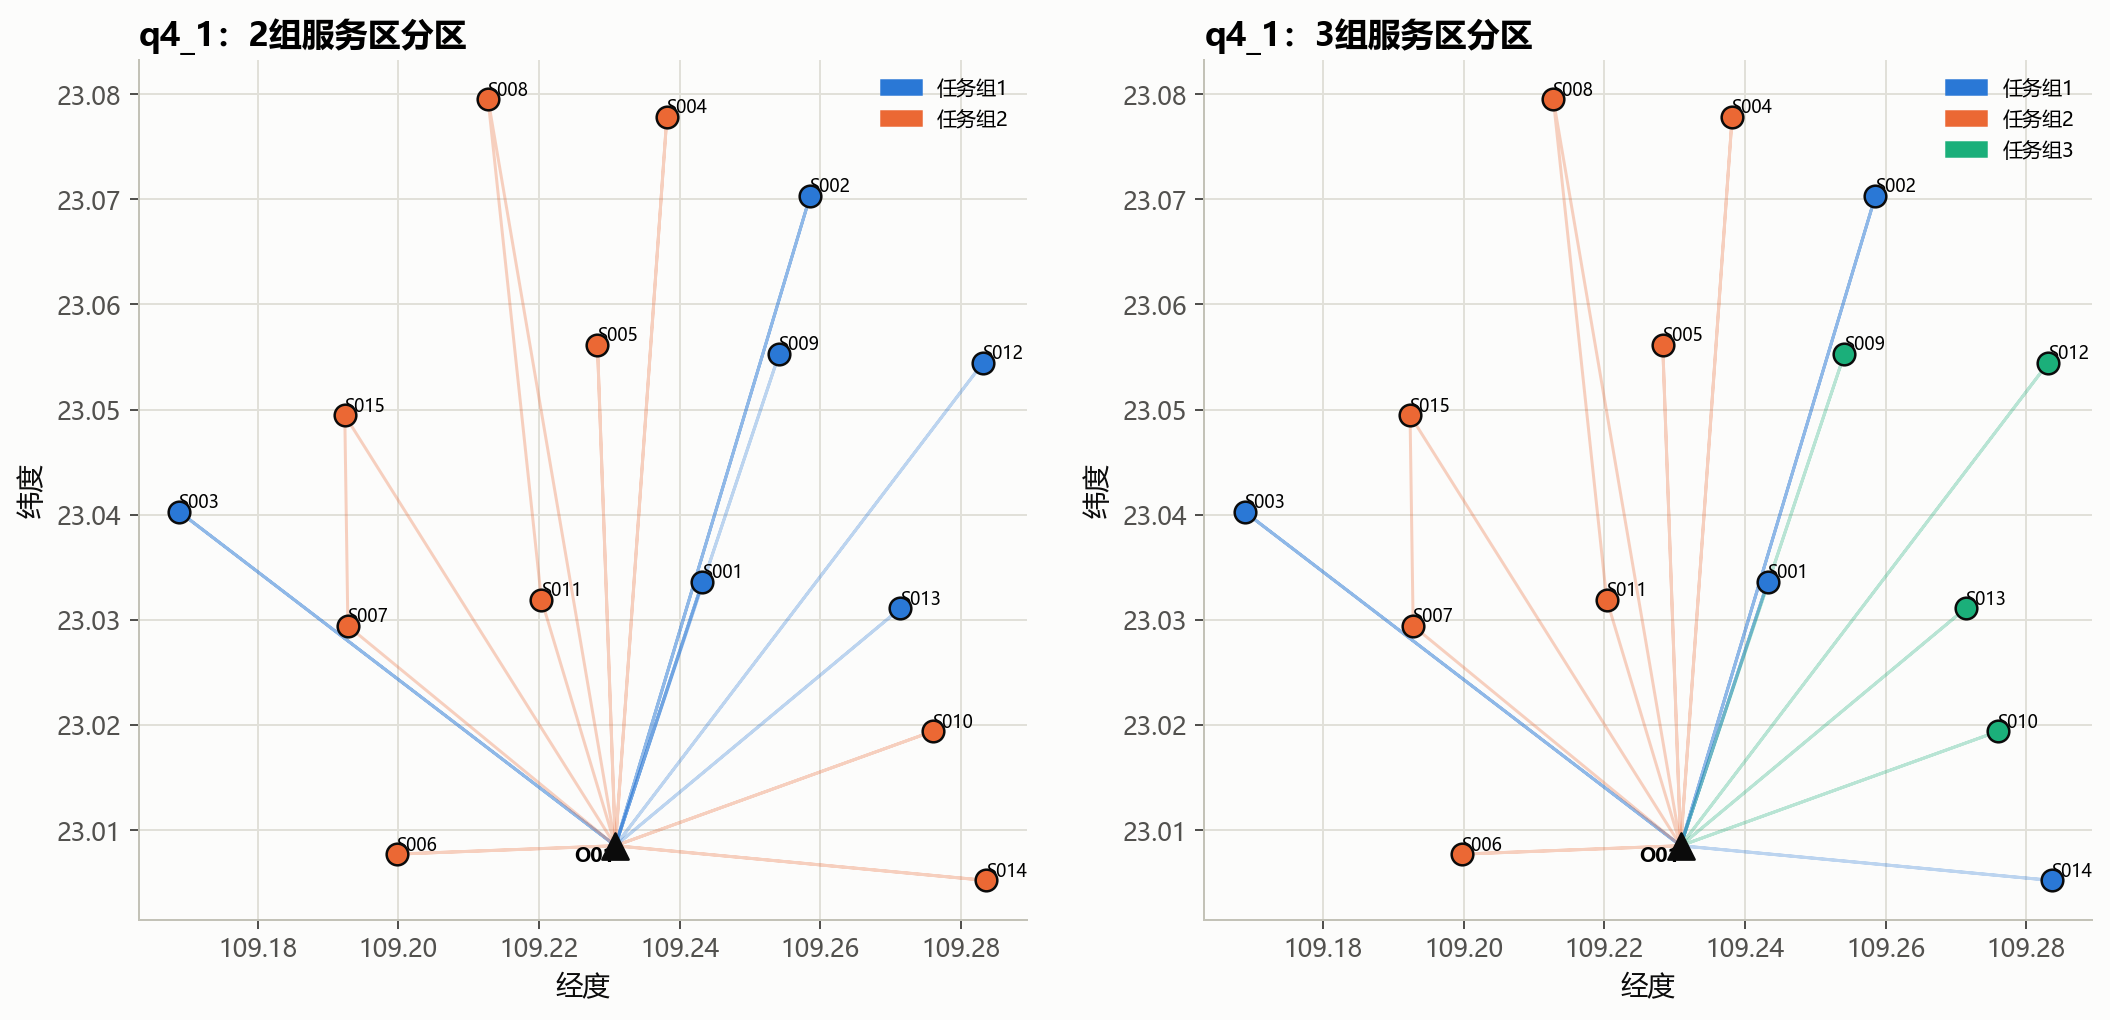
\includegraphics[width=0.62\textwidth]{figures/q4_1_01_分区地图.png}\label{fig:q4_main_map}}
\hfill
\subfloat[资源需求与库存]{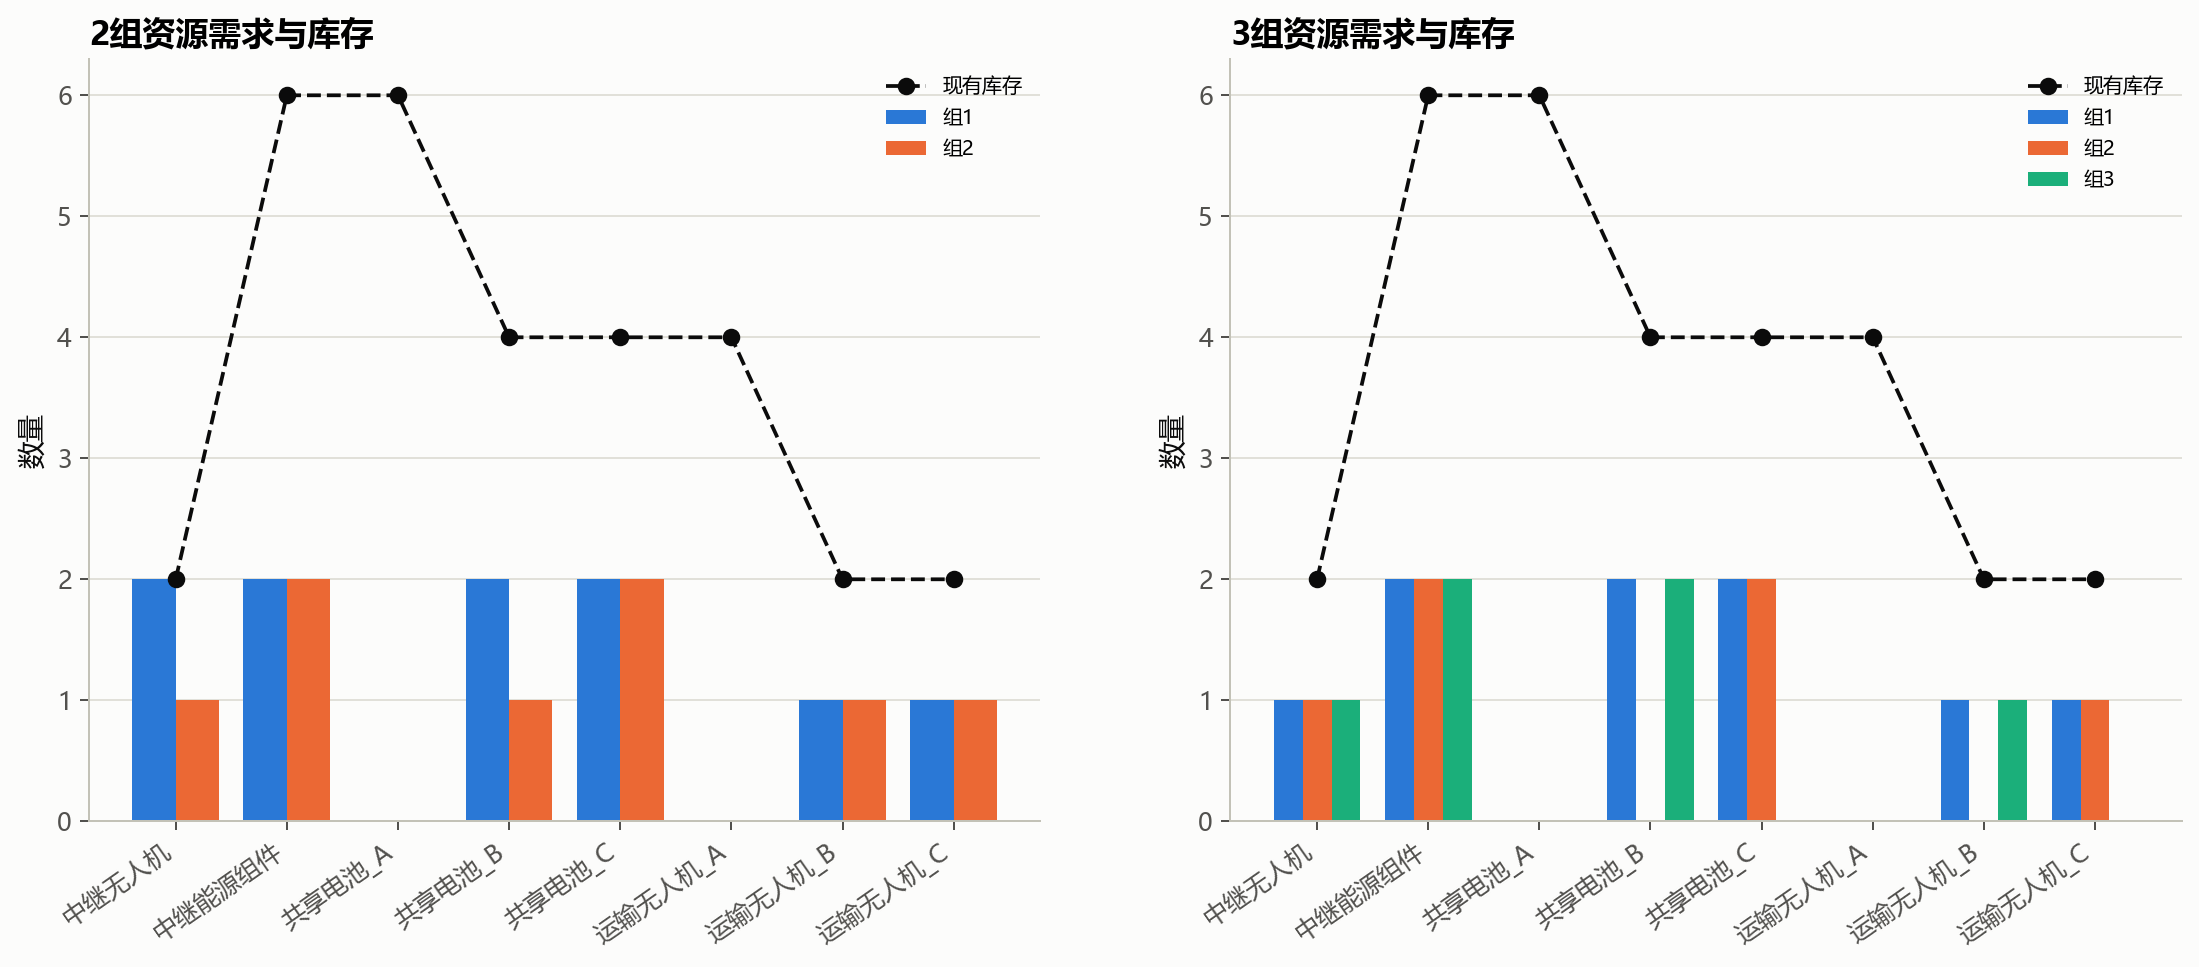
\includegraphics[width=0.36\textwidth]{figures/q4_1_02_资源需求库存.png}\label{fig:q4_main_res}}
\caption{问题四主方案（完全枚举）分区地图与资源需求}
\label{fig:q4_main_overview}
\end{figure}

图~\ref{fig:q4_main_map} 直观显示 K=2/K=3 的分区形态与任务块边界；图~\ref{fig:q4_main_res} 给出各组资源需求与库存对比，可见中继无人机在分组独立配置下需求超过库存，是缺口的唯一来源。图~\ref{fig:q4_main_bal} 给出主方案的组间工作量均衡与缺口冗余对比：K=2 时两组工作量接近（均衡系数 0.0337）、冗余较高；K=3 时三组工作量分化（均衡系数 0.3350）、冗余下降。K=2 与 K=3 的精确分区方案（各组服务区构成）分别见表~\ref{tab:q4_partition_k2} 与表~\ref{tab:q4_partition_k3}。

\begin{figure}[htbp]
\centering
\subfloat[组间工作量均衡]{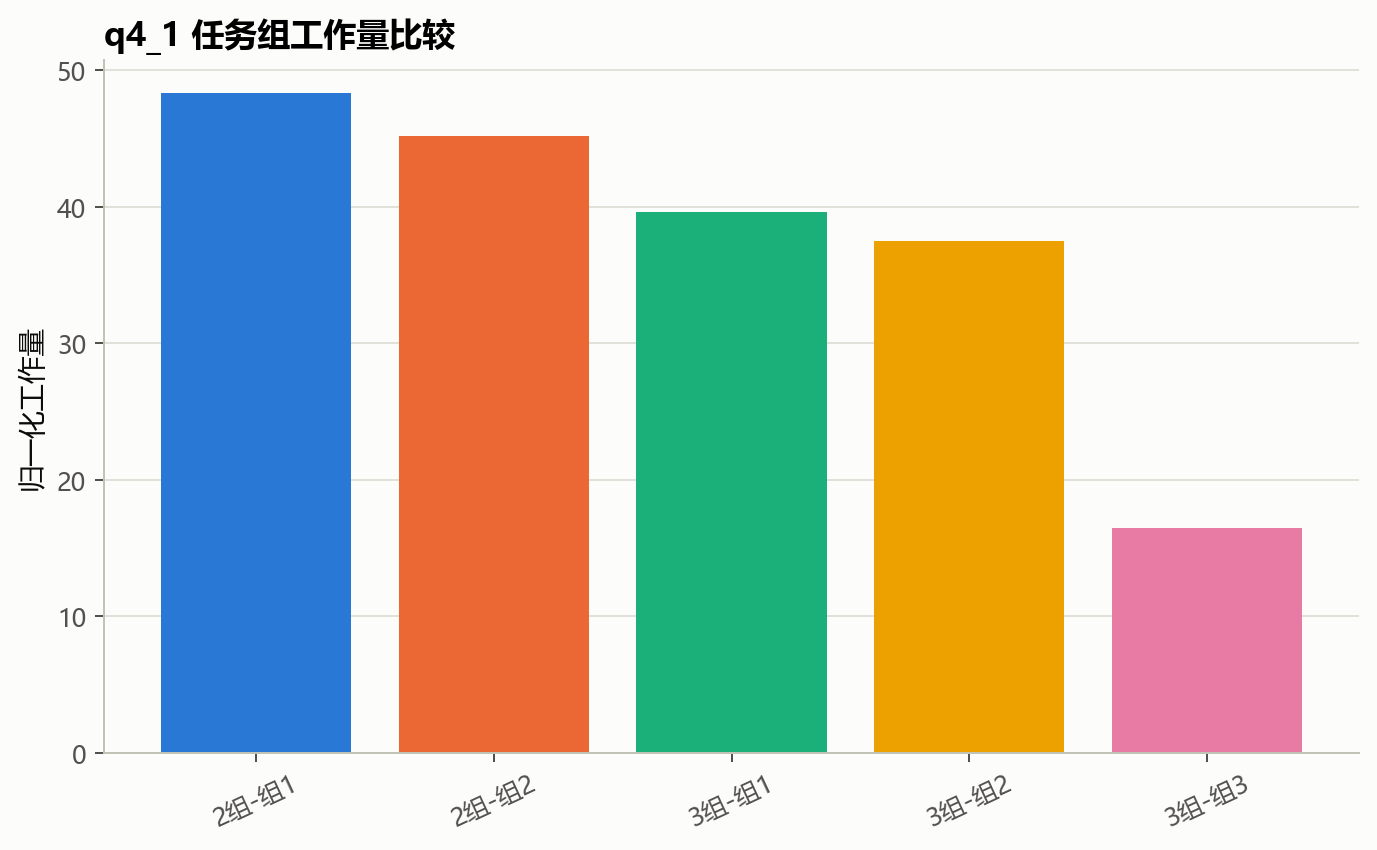
\includegraphics[width=0.48\textwidth]{figures/q4_1_03_工作量均衡.png}\label{fig:q4_main_bal}}
\hfill
\subfloat[资源缺口与冗余]{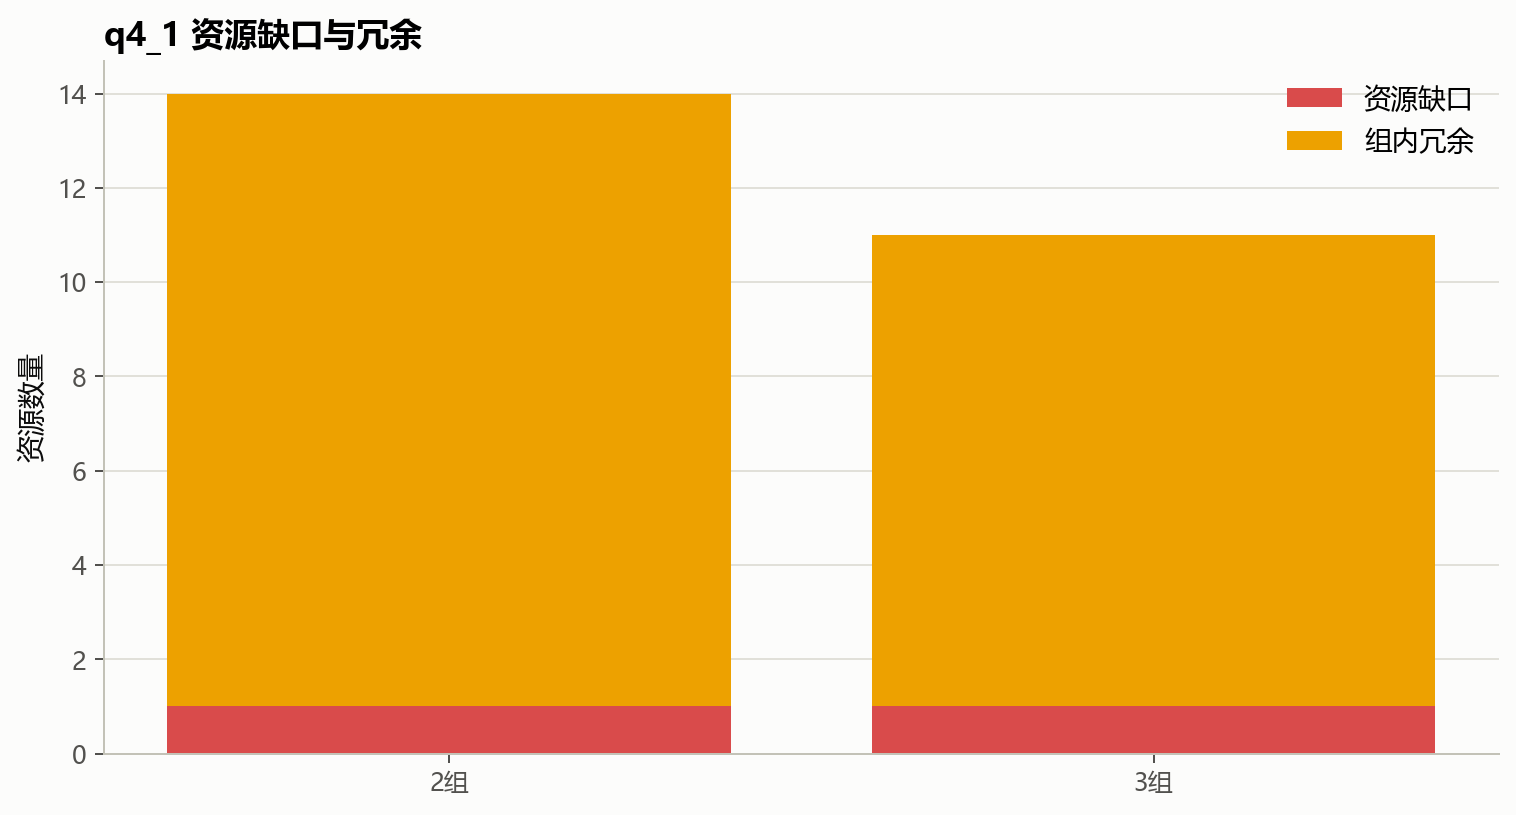
\includegraphics[width=0.48\textwidth]{figures/q4_1_04_缺口冗余.png}\label{fig:q4_main_gapred}}
\caption{问题四主方案（完全枚举）工作量均衡与缺口冗余}
\label{fig:q4_main_bal_overview}
\end{figure}

\begin{table}[htbp]
\centering\small
\caption{问题四精确枚举 K=2 分区方案}\label{tab:q4_partition_k2}
\begin{tabular}{cl}
\toprule 任务组 & 服务区 \\\midrule
1 & S001、S002、S003、S009、S012、S013 \\
2 & S004、S005、S006、S007、S015、S008、S011、S010、S014 \\\bottomrule\end{tabular}\end{table}


\begin{table}[htbp]
\centering\small
\caption{问题四精确枚举 K=3 分区方案}\label{tab:q4_partition_k3}
\begin{tabular}{cl}
\toprule 任务组 & 服务区 \\\midrule
1 & S001、S002、S003、S014 \\
2 & S004、S005、S006、S007、S015、S008、S011 \\
3 & S009、S010、S012、S013 \\\bottomrule\end{tabular}\end{table}


\subsection{对比方法：负载均衡初始化 + 模拟退火局部搜索}

对比方法（对应代码 \texttt{q4\_2.py}）采用局部搜索：以负载均衡（按作业时长 + 能耗 $\times$100 + 箱数 $\times$20 贪心）初始化分区，再以 300 轮模拟退火搜索（72\% 单块移动 / 28\% 两块交换），接受准则为标量得分 $score=10^6\,Gap+100\,\text{总规模}+10^4\,Bal+Red$ 的 Metropolis 判据，温度线性退火\cite{ref_sa}。该方法在任务块规模增大、完全枚举不可行时仍能给出可用解。

对比方法结果见表~\ref{tab:q4_enum} 与图~\ref{fig:q4_enum_overview}。K=2 得 2 组（组 1：S003、S005、S006、S009、S010、S013、S014；组 2：S001、S002、S004、S007、S008、S011、S012、S015），总规模 23、均衡系数 0.1480、冗余 10、缺口 3；K=3 得 3 组（组 1：S005、S007、S008、S010、S011、S014、S015；组 2：S001、S002、S004；组 3：S003、S006、S009、S012、S013），总规模 23、均衡系数 0.0299、冗余 11、缺口 4。

\begin{table}[htbp]
\centering
\caption{问题四对比方法（局部搜索）分区结果}
\label{tab:q4_enum}
\small
\begin{tabular}{lcccc}
\toprule
\textbf{分区} & \textbf{总规模} & \textbf{均衡系数} & \textbf{冗余} & \textbf{缺口} \\
\midrule
K=2 & 23 & 0.1480 & 10 & 3 \\
K=3 & 23 & 0.0299 & 11 & 4 \\
\bottomrule
\end{tabular}
\end{table}

\begin{figure}[htbp]
\centering
\subfloat[局部搜索分区地图]{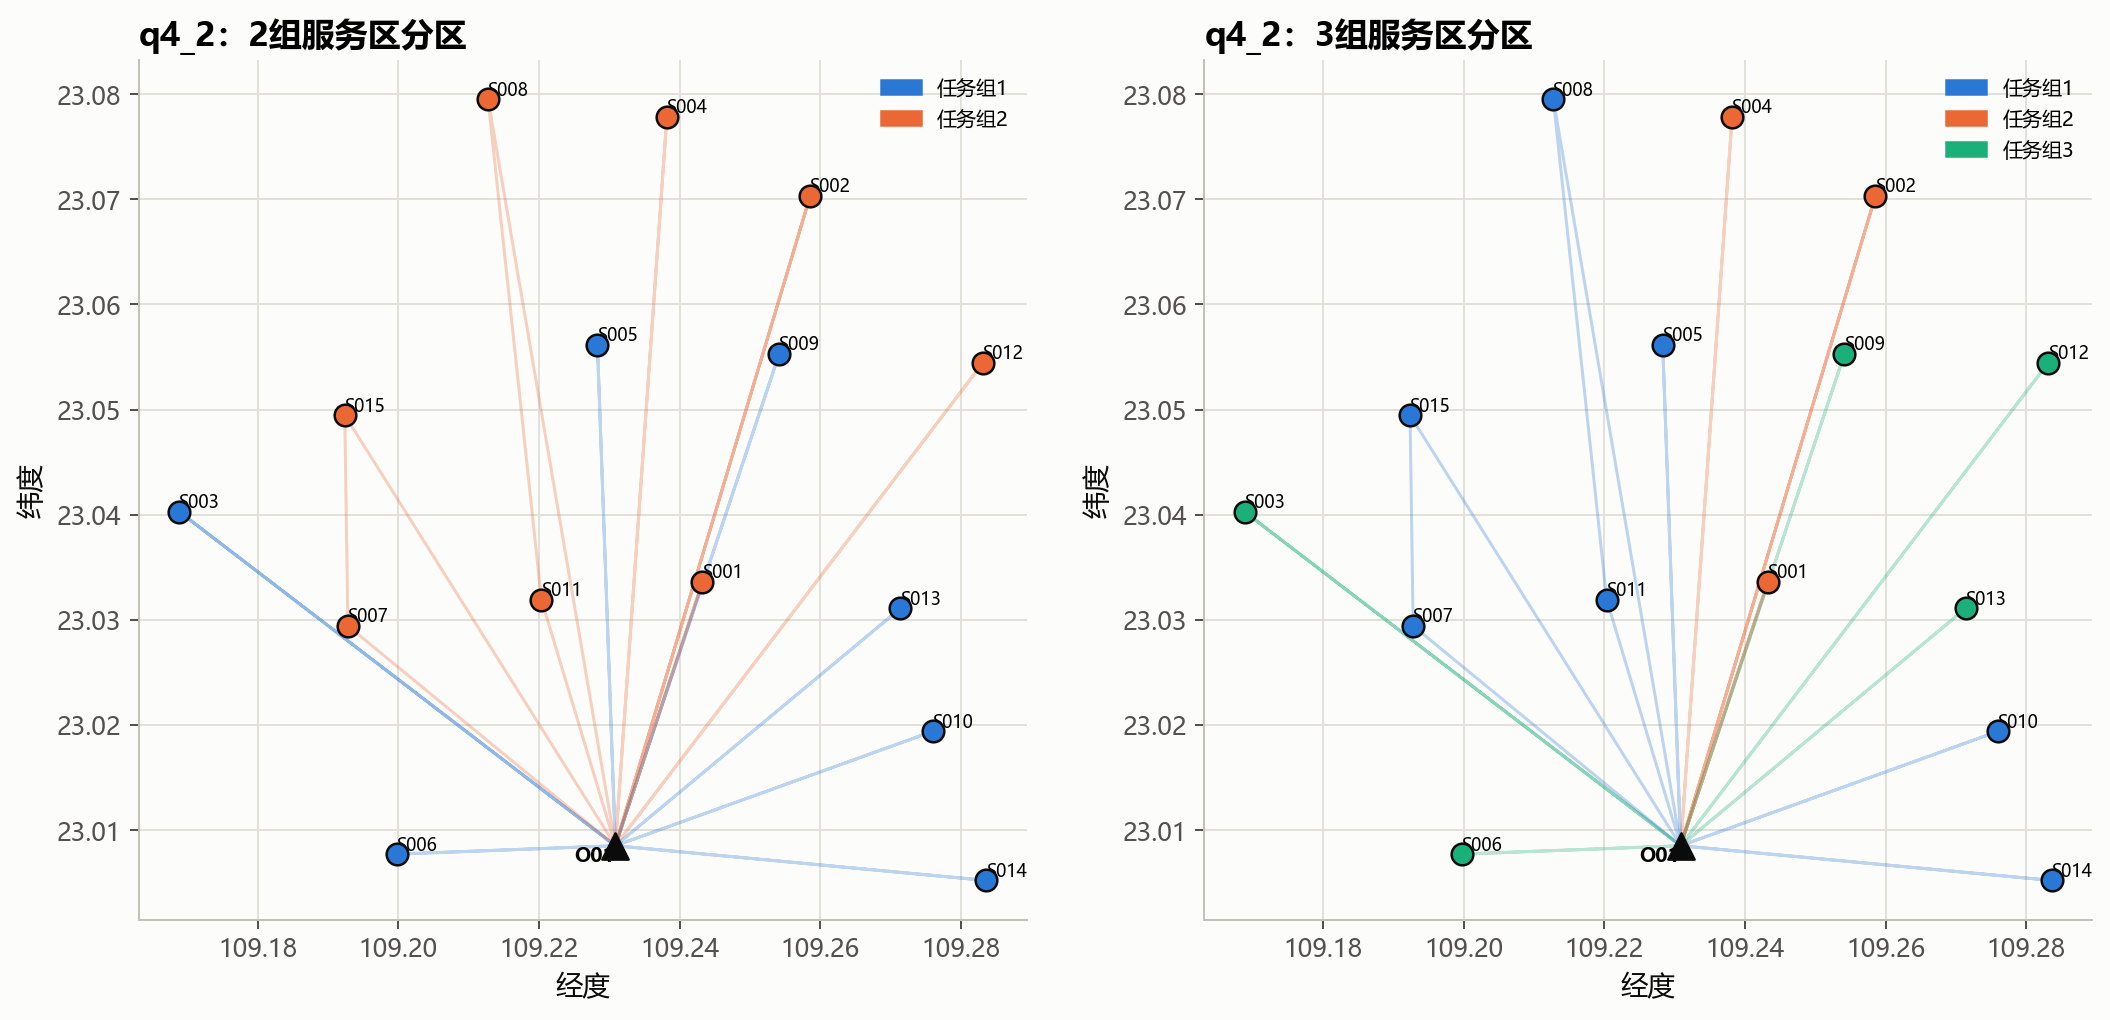
\includegraphics[width=0.62\textwidth]{figures/q4_2_01_分区地图.png}\label{fig:q4_enum_map}}
\hfill
\subfloat[资源需求与库存]{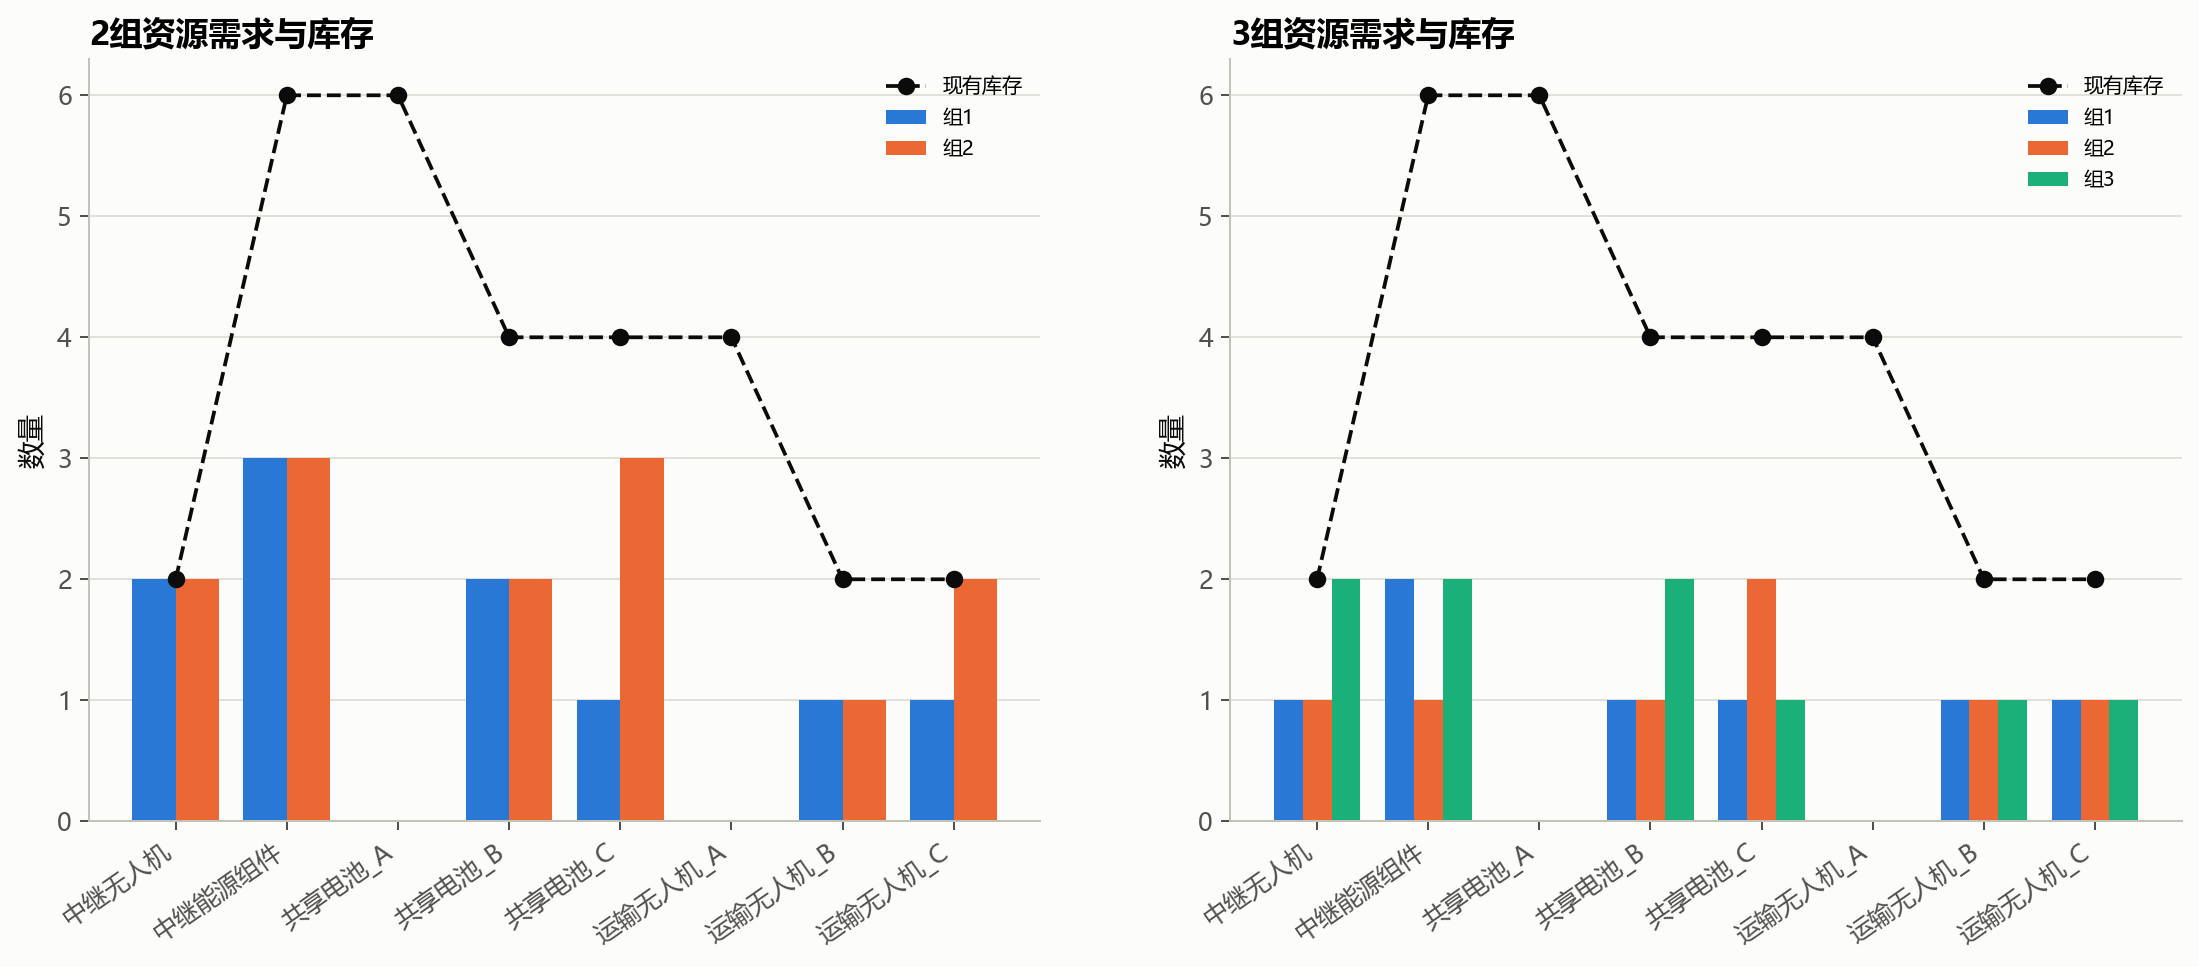
\includegraphics[width=0.36\textwidth]{figures/q4_2_02_资源需求库存.png}\label{fig:q4_enum_res}}
\caption{问题四对比方法（局部搜索）结果}
\label{fig:q4_enum_overview}
\end{figure}

\subsection{模型比对与资源缺口分析}

两种方法对比如表~\ref{tab:q4_compare} 与图~\ref{fig:q4_compare} 所示。完全枚举在 13 块规模内给出全局最优（缺口仅 1，来自中继无人机），但枚举规模随 $K$ 与块数呈 Bell 数增长（图~\ref{fig:q4_conv}），块数再增即不可行；局部搜索以可扩展的邻域搜索在 300 轮内收敛（图~\ref{fig:q4_conv} 显示其标量得分与缺口快速下降），K=3 组间均衡性较好（0.0299 优于枚举的 0.3350），但未收敛到全局最优，缺口更大（3/4）。

\begin{table}[htbp]
\centering
\caption{问题四两种方法结果对比}
\label{tab:q4_compare}
\small
\begin{tabular}{lcccc}
\toprule
\textbf{方案} & \textbf{总规模(K2/K3)} & \textbf{均衡(K2/K3)} & \textbf{缺口(K2/K3)} \\
\midrule
\textbf{完全枚举（主方案，精确）} & \textbf{18 / 21} & \textbf{0.0337 / 0.3350} & \textbf{1 / 1} \\
局部搜索（对比） & 23 / 23 & 0.1480 / 0.0299 & 3 / 4 \\
\bottomrule
\end{tabular}
\end{table}

\begin{figure}[htbp]
\centering
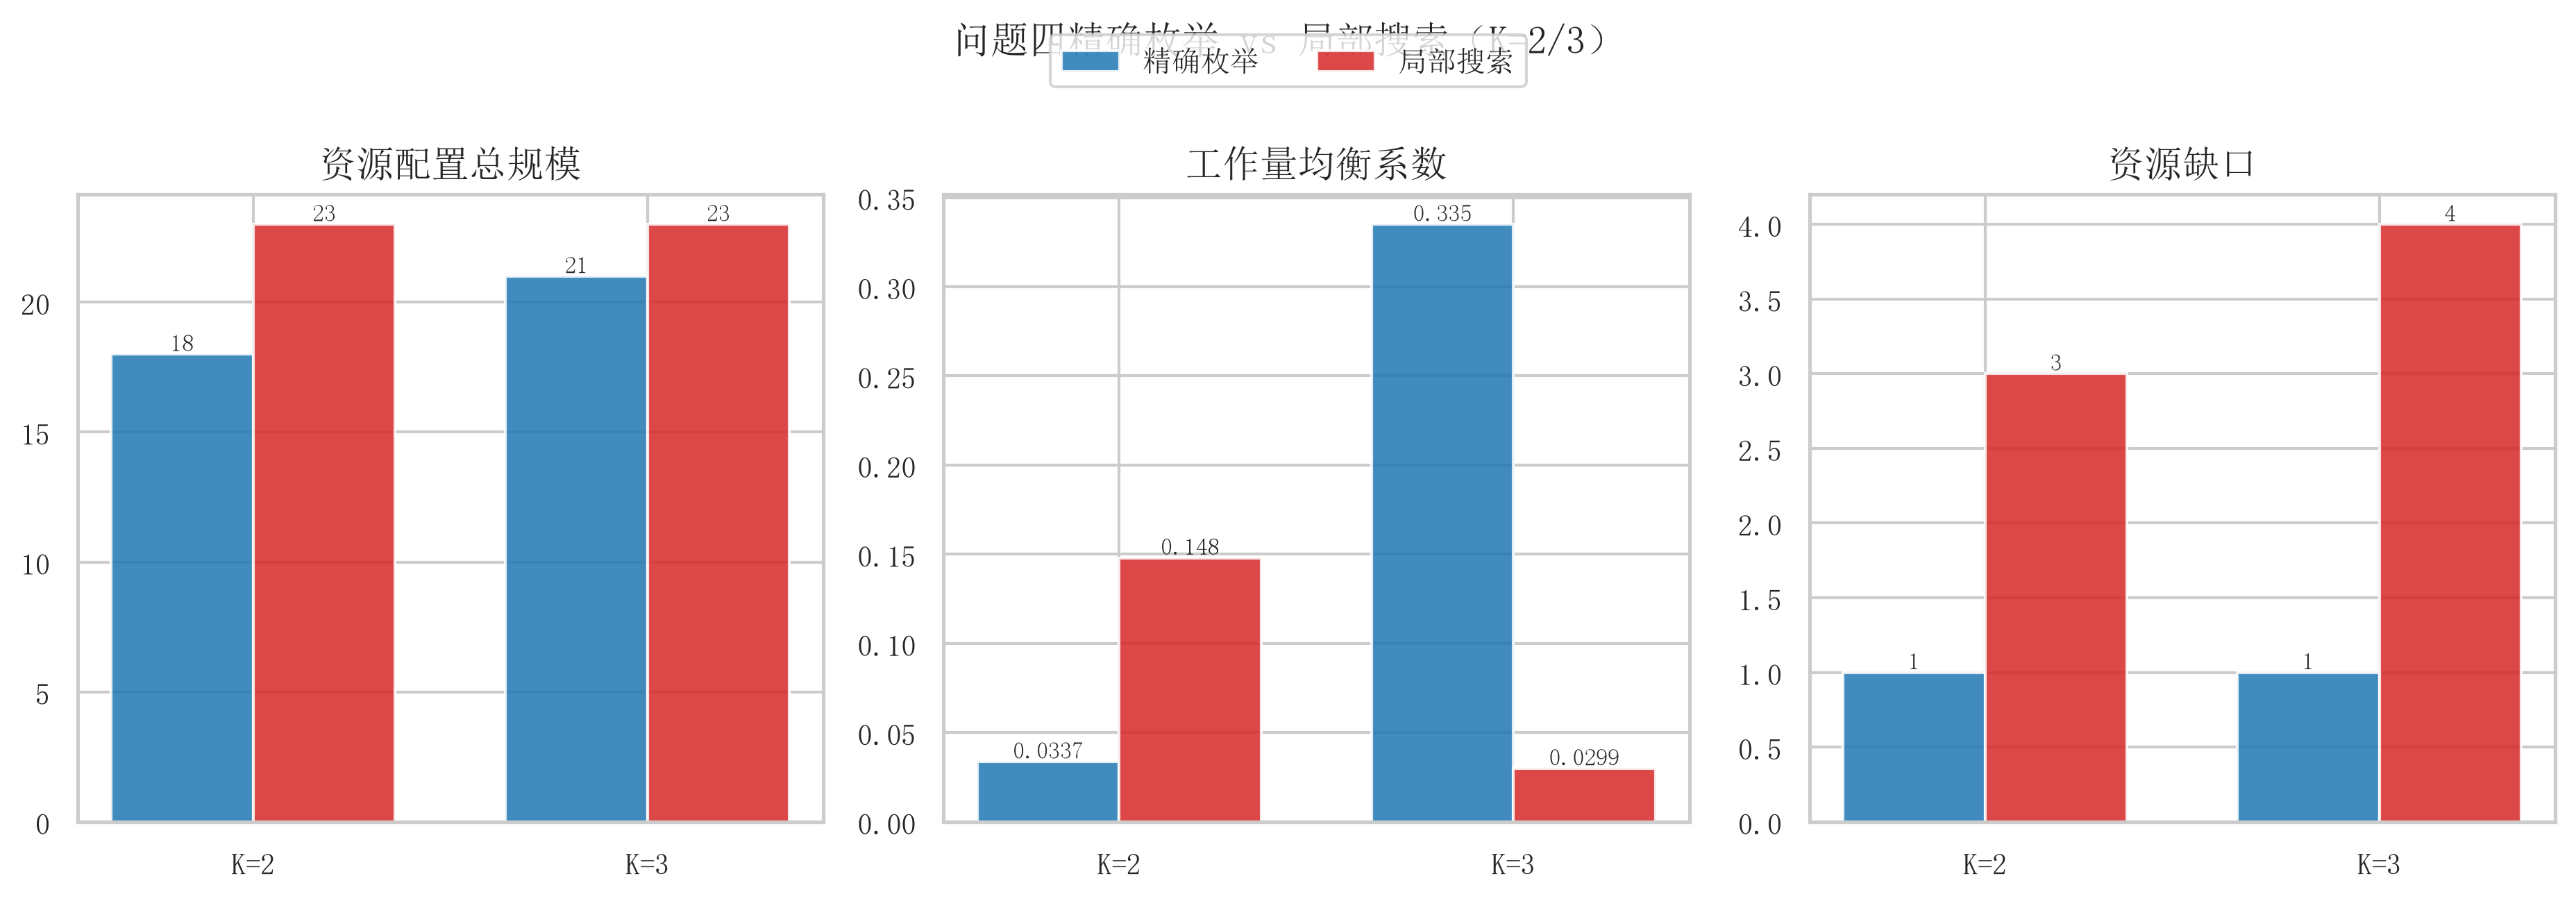
\includegraphics[width=0.95\textwidth]{figures/q4_extra_01_枚举vs局部搜索.png}
\caption{问题四精确枚举与局部搜索三维指标对比}
\label{fig:q4_compare}
\end{figure}

图~\ref{fig:q4_gap_heatmap} 以热力图给出精确枚举下各资源类型在 K=2/K=3 的缺口，可见缺口仅集中在中继无人机（各 1 个单位），其余运输机、共享电池、中继能源组件均无缺口，印证了"组间不共享"约束下中继机是唯一瓶颈的结论。

\begin{figure}[htbp]
\centering
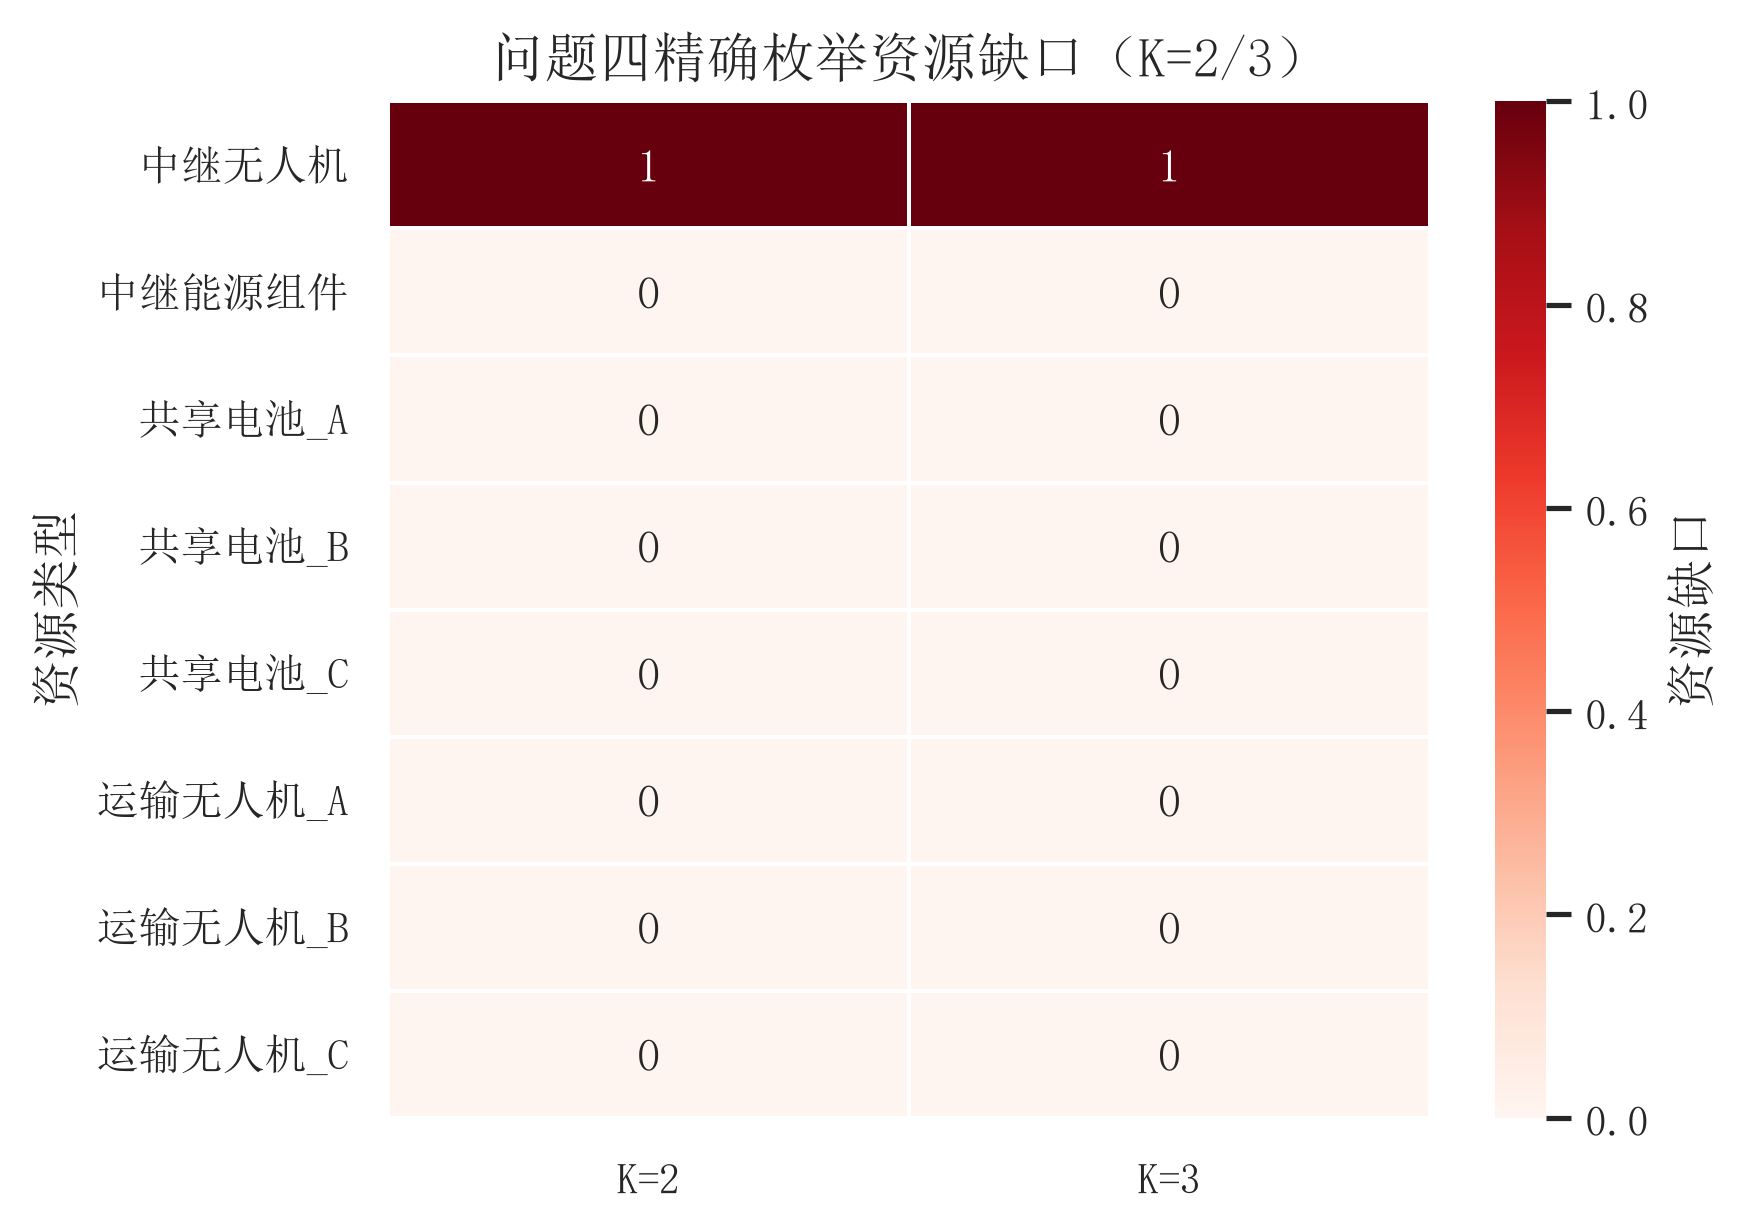
\includegraphics[width=0.55\textwidth]{figures/q4_extra_04_资源缺口热力图.png}
\caption{问题四精确枚举资源缺口热力图}
\label{fig:q4_gap_heatmap}
\end{figure}

\textbf{资源缺口的成因}：两种方法均出现中继无人机缺口——各组独立配置时，中继无人机的 K 组峰值需求之和（3--4）超过现有库存 2，但各组单独看峰值需求都不超库存，即"组间不共享"这一约束本身带来的资源代价，并非某组用量异常。局部搜索额外的运输 C/B 型缺口同理：分组越多，各组须各自留出峰值冗余，同一批次的架次被拆到不同组后无法互相借用资源，总需求规模随 $K$ 增大而上升。

\begin{figure}[htbp]
\centering
\subfloat[局部搜索收敛过程]{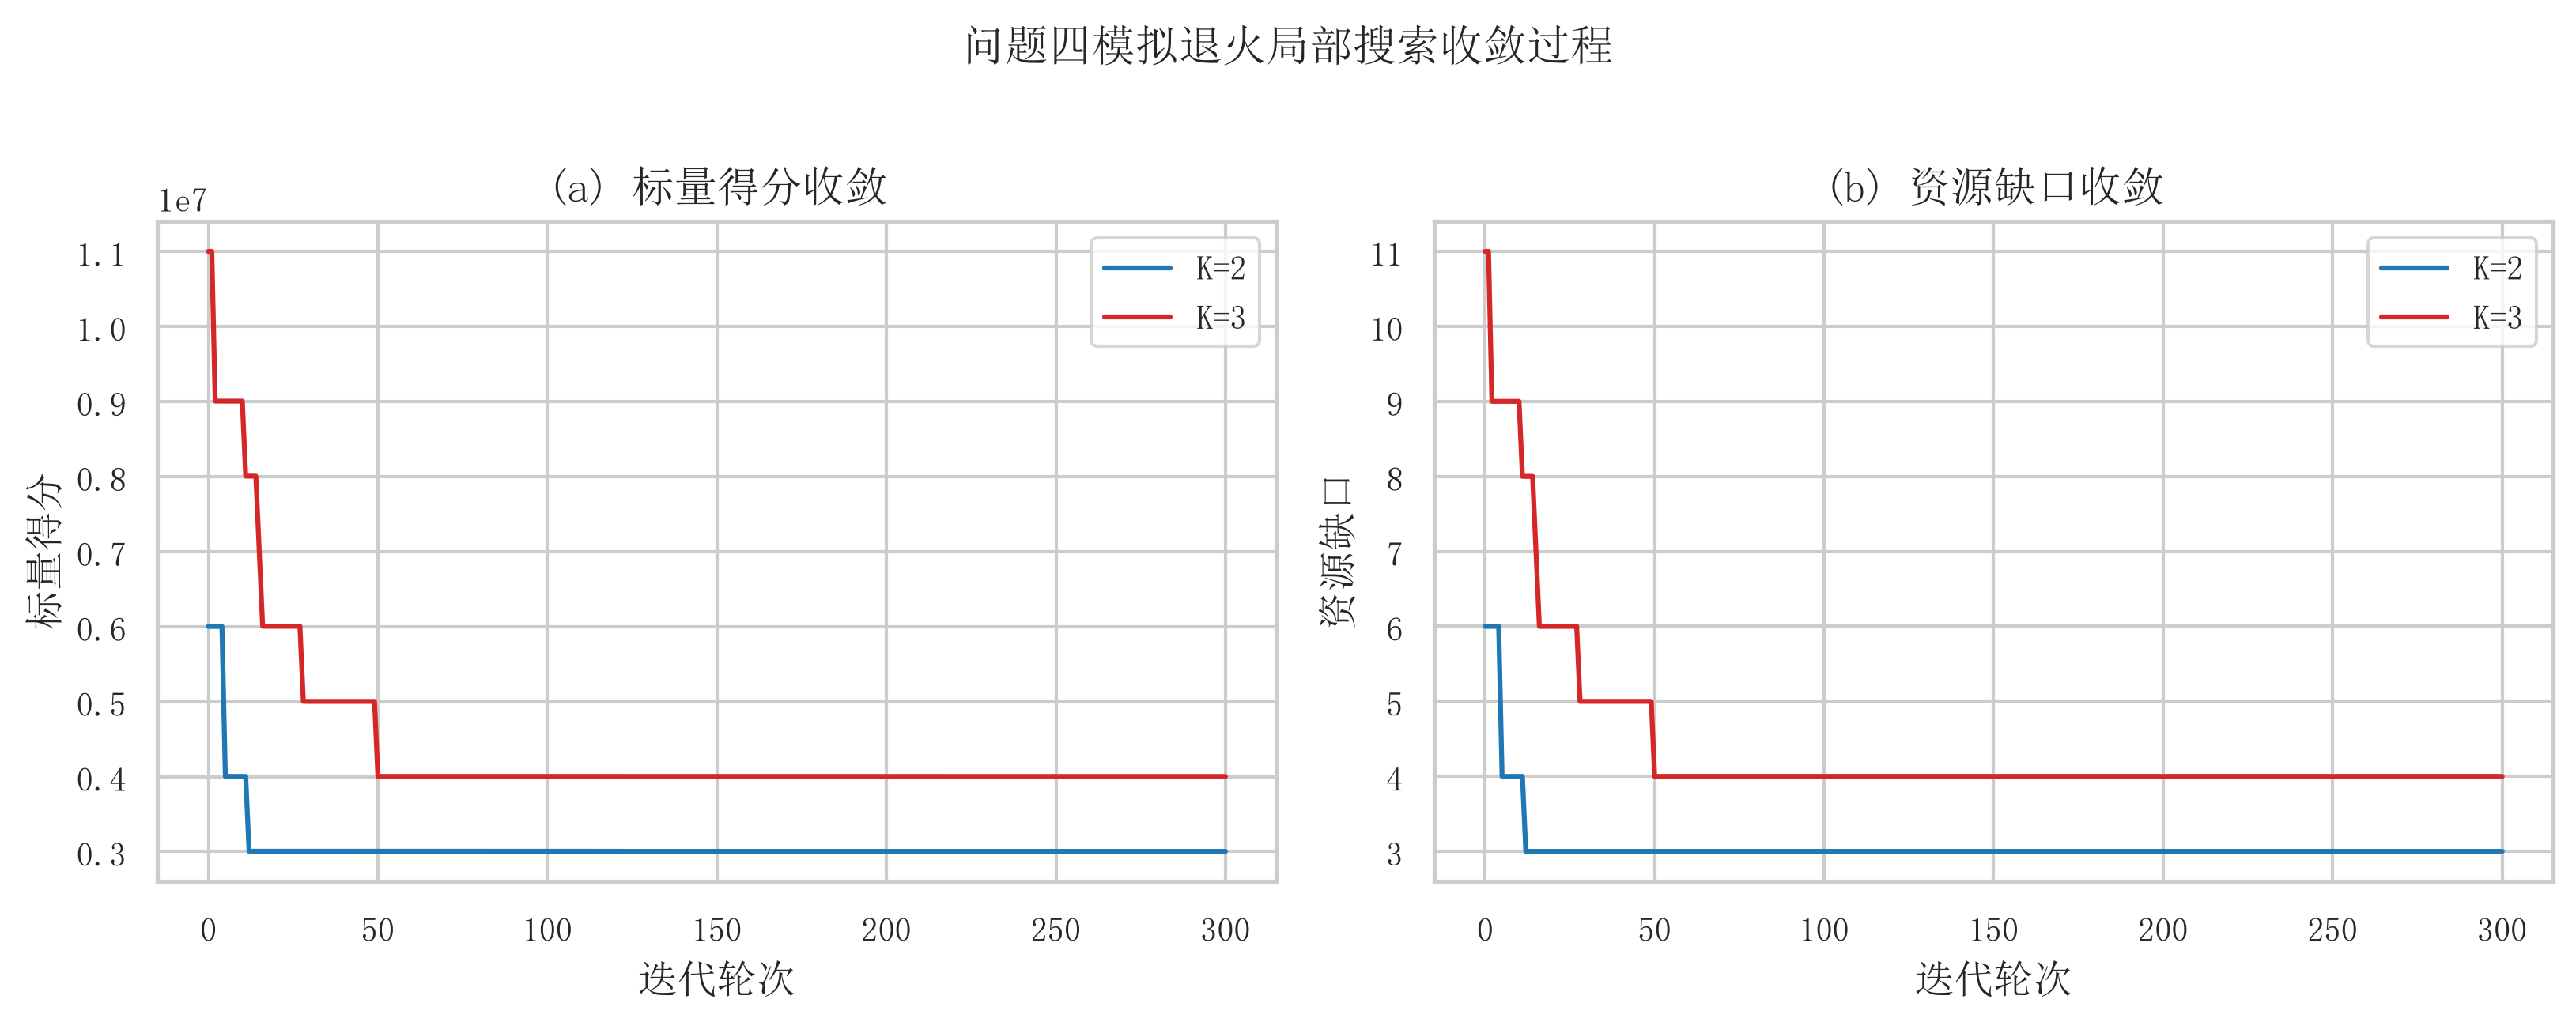
\includegraphics[width=0.48\textwidth]{figures/q4_extra_02_SA收敛曲线.png}\label{fig:q4_conv_sa}}
\hfill
\subfloat[枚举复杂度随 K 增长]{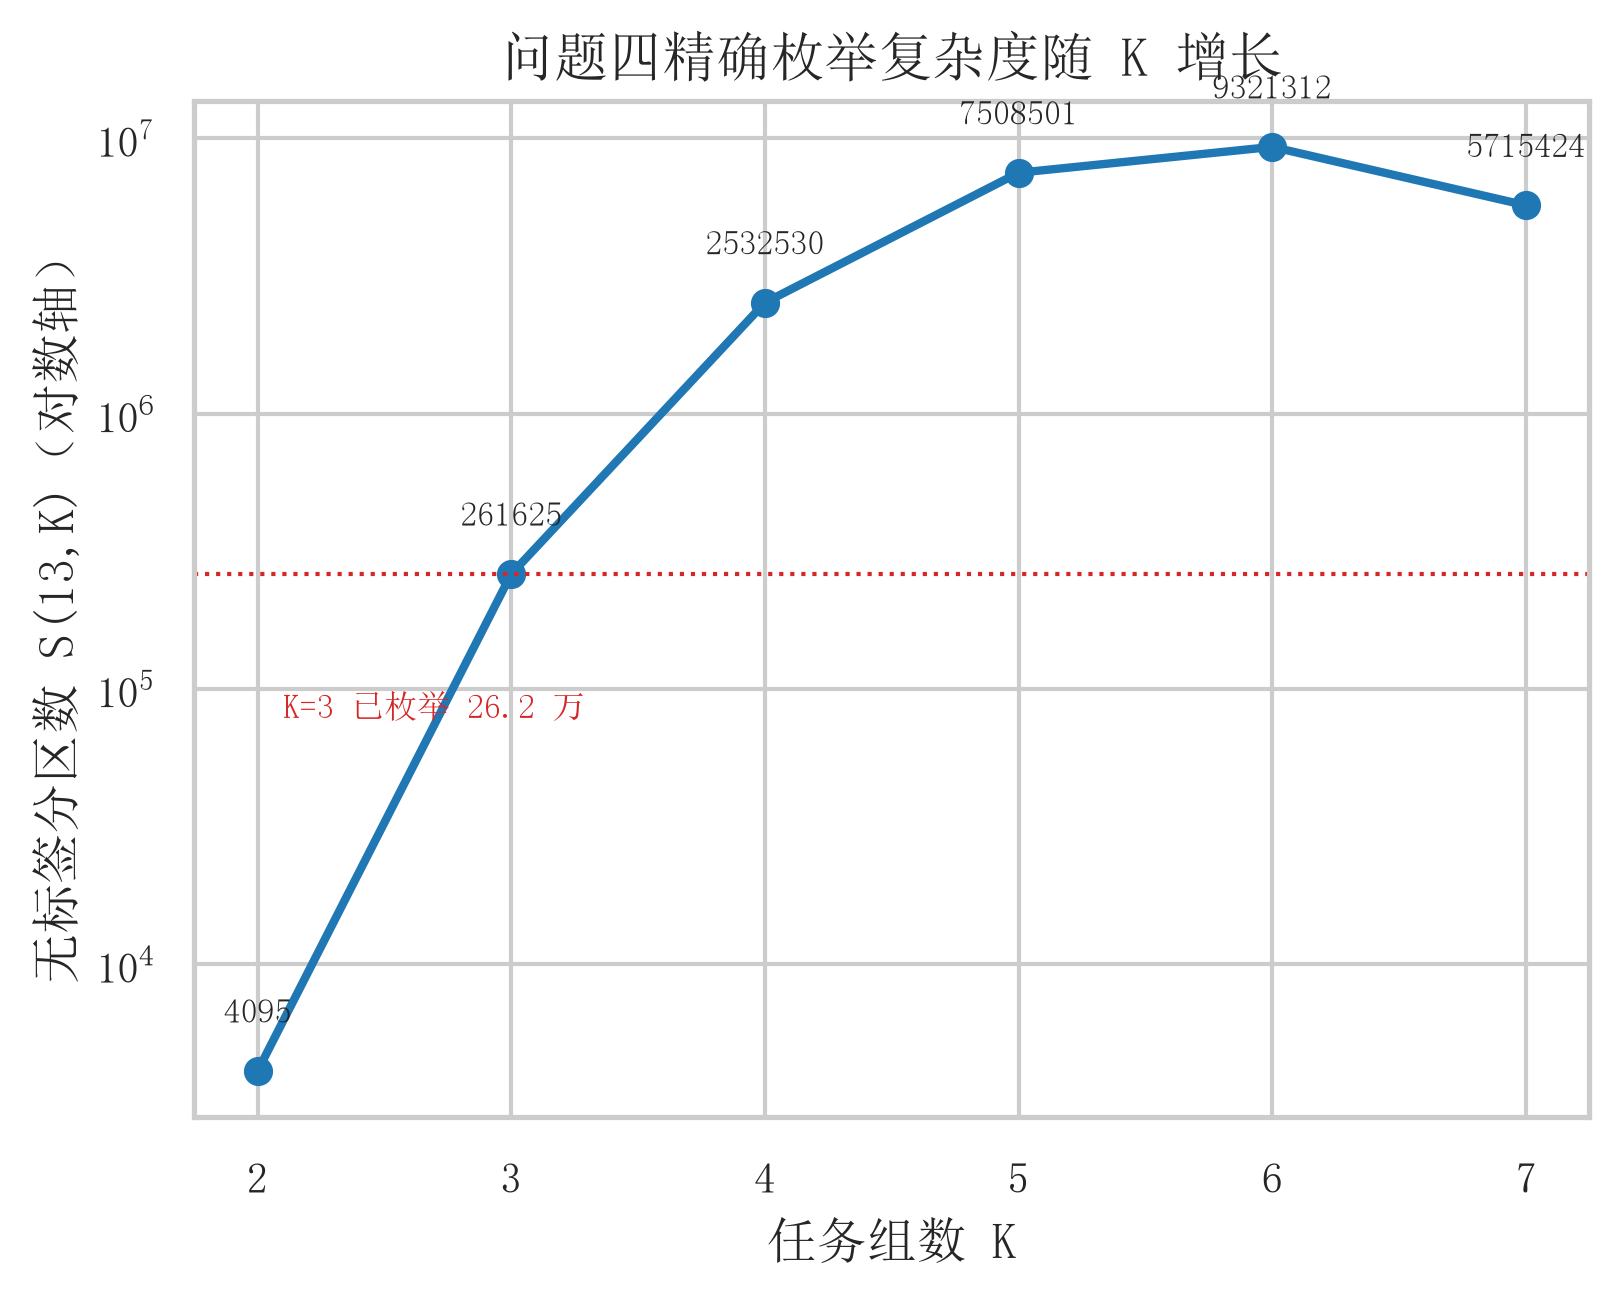
\includegraphics[width=0.48\textwidth]{figures/q4_extra_03_枚举复杂度.png}\label{fig:q4_conv}}
\caption{问题四局部搜索收敛与精确枚举复杂度}
\label{fig:q4_conv_overview}
\end{figure}

综合而言，精确枚举在给定 13 块规模下资源代价最小（缺口 1），是"资源配置最优"的严格全局解，故本文以完全枚举为主方案；局部搜索在均衡性上表现更好、且能扩展到完全枚举不可行的更大规模，作为可扩展性的对比方法，两者缺口差异被如实报告、不粉饰。
